\documentclass[a4paper, 12pt]{article}

\usepackage[slovene]{babel}
\usepackage[utf8]{inputenc}
\usepackage[T1]{fontenc}
\usepackage{lmodern}
\usepackage{units}
\usepackage{eurosym}
\usepackage{amsmath}
\usepackage{amssymb}
\usepackage{amsthm}
\usepackage{amsfonts}
\usepackage{mathtools}
\usepackage{graphicx}
\usepackage{color}
%\usepackage{url}
\usepackage{hyperref}
\usepackage{enumerate}
\usepackage{enumitem}
\usepackage{pifont}
\usepackage{tikz-cd}
\usetikzlibrary{babel}
\usepackage{adjustbox}
\usepackage{stmaryrd}

% set margin and layout here
\usepackage[margin=0.5in]{geometry}

% commonly used math operators
\DeclareMathOperator{\diam}{diam}
\DeclareMathOperator{\rank}{rank}
\DeclareMathOperator{\im}{im}
\DeclareMathOperator{\coker}{coker}
\DeclareMathOperator{\Lin}{Lin}
\DeclareMathOperator{\Ann}{Ann}
\DeclareMathOperator{\Ass}{Ass}
\DeclareMathOperator{\Spec}{Spec}
\DeclareMathOperator{\mSpec}{mSpec}
\DeclareMathOperator{\Quot}{Quot}
\DeclareMathOperator{\Tor}{Tor}
\DeclareMathOperator{\Ext}{Ext}
\DeclareMathOperator{\Hom}{Hom}
\DeclareMathOperator{\pr}{pr}

% commonly used math objects
\newcommand{\D}{\mathbb{D}}
\renewcommand{\S}{\mathbb{S}}
\newcommand{\B}{\mathbb{B}}
\newcommand{\N}{\mathbb{N}}
\newcommand{\Z}{\mathbb{Z}}
\newcommand{\Q}{\mathbb{Q}}
\newcommand{\R}{\mathbb{R}}
\newcommand{\C}{\mathbb{C}}
\renewcommand{\P}{\mathbb{P}}
\newcommand{\I}{\mathbb{I}}

% commonly used math relations
\newcommand{\iso}{\cong}
\newcommand{\homeo}{\approx}
\newcommand{\htpeq}{\simeq}
\newcommand{\hlgeq}{\sim}
\newcommand{\idtfy}{\longleftrightarrow}

% commonly used math symbols
\newcommand{\closure}[1]{\overline{#1}}
\newcommand{\subideal}{\vartriangleleft}
\newcommand{\supideal}{\vartriangleright}

% title data - MODIFY
\title{Algebraična topologija 1 - izpitna domača naloga}
\author{Benjamin Benčina, 27192018}

\begin{document}

\maketitle

\underline{\textbf{Nal. 1:}}
\begin{enumerate}[label=(\alph*)]
	\item Pokažimo, da je množica $\sqcup_{n=1}^\infty G_n$ diskretna v $V$. To je po definiciji res, ko je vsaka njena podmnožica odprta, kar pa je ekvivalentno temu, da je vsaka množica $A \subseteq \sqcup_{n=1}^\infty G_n$ zaprta. Množica $A$ je zaprta v inducirani (šibki) topologijo natanko tedaj, ko je $A \cap W$ zaprta za vsak končnorazsežen vektorski podprostor $W \leq V$. Vsak tak $W$ je oblike $W = \bigoplus_{i = 1}^n \Lin(H_{k_i})$, kjer so vse $H_{k_i} \subseteq G_{k_i}$ končne množice. Od tod sledi, da je $A \cap W \subseteq \sqcup_{i=1}^n H_{k_i} \subseteq \sqcup_{i=1}^n G_{k_i}$ končna. Množica $A \cap H_{k_i}$ je po definiciji linearne topologije zaprta v $\Lin(G_{k_i})$, zato je tudi $A \cap W = \sqcup_{i=1}^n A \cap H_{k_i}$ zaprta.
	
	\item Pokažimo, da je družina $\lbrace G_i \rbrace$ spojljiva.
	
	Uporabimo definicijo spojljivosti iz navodil. Naj bo $\Sigma_{n = 1}^\infty t_n g_n = \Sigma_{n = 1}^\infty s_n h_n$ (končne vsote). Ker je $G$ (abstraktna) baza, je $t_n = s_n$ za vsak $n \in \N$. Če $t_n > 0$, nam zvezno množenje z $\frac{1}{t_n}$ da $g_n = h_n$. Obratna implikacija je očitna.
	
	\item Identficirajmo prostor $E\Z_2$.
	
	Hitro vidimo $\Z_2 * \Z_2 \homeo \S^1$, $\Z_2 * \Z_2 * \Z_2 \homeo \S^2$ in tako dalje, kar nam v limiti da $E\Z_2 \homeo \S^\infty$.
	
	\begin{figure}[h]
		\centering
		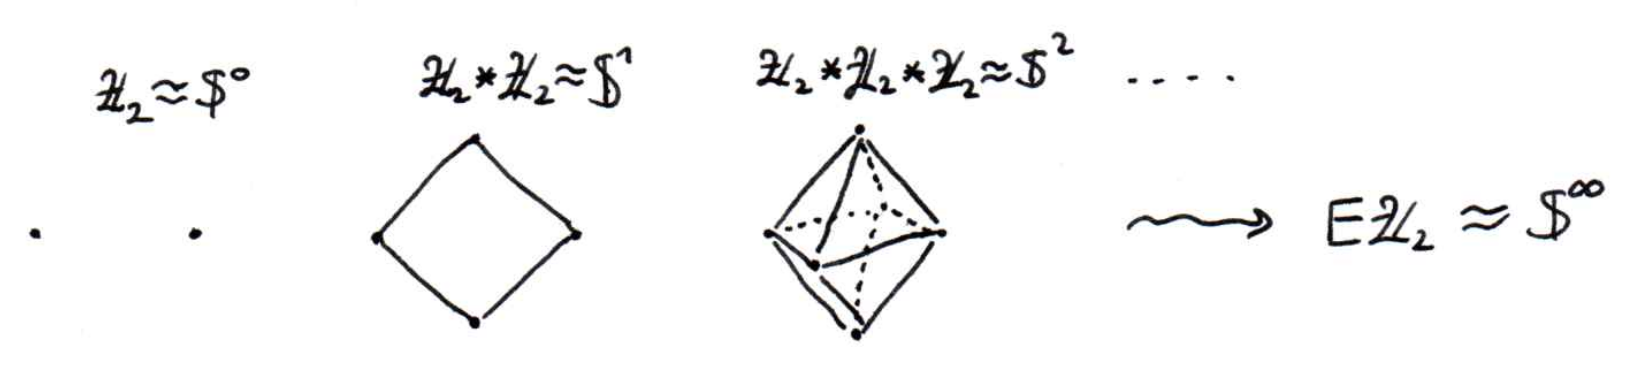
\includegraphics[scale=0.3]{EZ1c.png}
		\caption{Induktivno konstruiramo $E\Z_2$}
		\label{fig:EZ2}
	\end{figure}
	
	\item Dokažimo, da je prostor $EG$ zaprt v $V$.
	
	To je res natanko tedaj, ko je $EG \cap W$ zaprt za vsak končnorazsežen vektorski podprostor $W \leq V$, kar je res natanko tedaj, ko je $*_{i = 1}^nH_i$ zaprta v $V$ za neke končne podmnožice $H_i \subseteq G_i$, kar pa je res natanko tedaj ko je končna množica $H$ zaprta v $V$, to pa je res po definiciji linearne topologije (vsaka končna množica je vsebovana v nekem končno razsežnem podprostoru).
	
	\item Naj bodo $1 \leq i_0 < i_1 < \cdots < i_n < \infty$ naravna števila in naj $g_{i_k} \in G_{i_k}$ tvorijo poljubno $(n+1)$-terico. Definiramo (odprto) $n$-celico
	\[
	e(i_0, \dots, i_n ; \; g_{i_0}, \dots, g_{i_n}) = \lbrace \Sigma_{k = 0}^n t_{i_k}g_{i_k}; \; \forall k: t_{i_k} > 0, \; \Sigma_{k = 0}^nt_{i_k} = 1 \rbrace \subset EG
	\]
	z zaprtjem $[g_{i_0}, \dots, g_{i_n}],^{i_0, \dots, i_n}$. Dokažimo, da ima $EG$ šibko topologijo glede na družino zaprtih celic.
	
	Vemo že, da ima $EG$ šibko topologijo glede na vse končno razsežne vektorske podprostore $W \leq V$. Očitno je tudi $[g_{i_0}, \dots, g_{i_n}],^{i_0, \dots, i_n}$ zaprta v vsakem $W$, ki jo vsebuje. Zato vzemimo množico $A \subset EG$.
	Za prvo implikacijo privzemimo, da je $A$ zaprta v $EG$. Po definiciji šibke topologije gleda na končno razsežne podprostore je $A \cap W$ zaprta množica za vse končno razsežne podprostore $W \leq V$. Potem pa je tudi $A \cap [g_{i_0}, \dots, g_{i_n}],^{i_0, \dots, i_n}$ zaprta za vsako zaprto celico, ki je vsebovana v $W$. Ker je vsaka zaprta celica vsebovana v nekem končno razsežnem podprostoru, konkretno v $\oplus_{k=0}^n\Lin(\lbrace g_{i_k} \rbrace)$, je implikacija dokazana.
	Za drugo smer privzemimo, da je $A \cap [g_{i_0}, \dots, g_{i_n}],^{i_0, \dots, i_n}$ zaprta za vsako zaprto $n$-celico za vsak $n \in \N$. Vendar ker je $A \subseteq EG$, je $A \cap W$ za nek končno razsežen vektorski podprostor $W \leq V$ točno $A \cap [g_{i_0}, \dots, g_{i_n}],^{i_0, \dots, i_n}$ za neko zaprto $n$-celico. Sledi, da je $A\cap W$ zaprta za vsak končno razsežen vektorski podprostor $W \leq V$, torej je po definiciji šibke topologije (prvotne) $A \subset EG$ zaprta.
	Preverili smo definicijo šibke topologije na $EG$ glede na zaprte celice.
	
	\item Pokažimo, da je s predpisom $\tau_j(\Sigma_{n = 1}^\infty t_ng_n) = t_j$ definirana zvezna preslikava $EG \to [0, 1]$.
	
	Preslikava $\tau_j$ je kompozitum zvezne projekcije $\pr_j$ in množenja z $g_j^{-1}$, ki je zvezno po definiciji linearne topologije. Torej je $\tau_j =i_1 \circ \mu_{g_j^{-1}}\circ\pr_j$ zvezna kot kompozitum zveznih preslikav, kjer je $i_1$ inverz naravne vložitve $t \mapsto t\cdot 1$.
	
	\item Naj bo $S_j = \tau_j^{-1}((0, 1])$. Na $S_j$ je potem dobro definirana preslikava $p_j(\Sigma_{n = 1}^\infty t_ng_n) = g_j$. Pokažimo, da je $p_j \colon S_j \to G_j \equiv G$ zvezna.
	
	Preslikava $p_j$ je kompozitum $\pr_j$ in množenja z $\frac{1}{t_j}$, ki je zvezno po definiciji linearne topologije. Torej je $p_j = i_2 \circ m_{\frac{1}{t_j}} \circ \pr_j$ zvezna kot kompozitum zveznih preslikav, kjer je $i_2$ inverz naravne vložitve $g \mapsto 1 \cdot g$.
	
	\item Dokažimo, da ima $EG$ strukturo CW-kompleksa, v katerem so odprte celice natanko tiste iz točke (e).
	
	Za karakteristične preslikave vzemimo kar identične afine preslikave
	\[
	\Phi_{i_0, \dots, i_n; g_{i_0}}, \dots, g_{i_n}^{(n)} \colon [g_{i_0}, \dots, g_{i_n}]^{i_0, \dots, i_n} \to EG.
	\]
	Preverimo z alternativno definicijo CW-kompleksa. Prostor $EG$ je očitno Hausdorffov, vse zožitve karakterističnih preslikav na odprte celice so kot identične preslikave injektivne. Po konstrukciji prostora $EG$ je  $EG$ ravno disjunktna unija vseh odprtih celic, saj iz definicije celic takoj sledi, da sta nedisjunktni celici enaki. Definicija celice nam prav tako zagotovi, da je rob vsake $n$-celice unija končno mnogo odprtih celic nižje dimenzije, saj je vsaka vsebovana v končno razsežnem vektorskem prostoru, njen rob pa je sestavljen iz točno $(n+1)$ mnogo $(n-1)$-celic (nadaljujemo induktivno do dimentize $0$ in dobimo končnost). Pogoj šibke topologije glede na celice smo preverili v točki (e).
	
	\item Naj bo $G \times EG \to EG$ preslikava, definirana s predpisom $(g, \Sigma_{n = 1}^\infty t_n g_n) \mapsto \Sigma_{n = 1}^\infty t_n (gg_n)$. Prepričajmo se, da je to levo delovanje diskretne grupe $G$ na prostor $EG$.
	
	Računamo
	\begin{align*}
	&(1, \Sigma_{n = 1}^\infty t_ng_n) \mapsto \Sigma_{n = 1}^\infty t_n(1g_n) = \Sigma_{n = 1}^\infty t_ng_n\\
	& (h, (g, \Sigma_{n = 1}^\infty t_ng_n)) \mapsto (h, \Sigma_{n = 1}^\infty t_n(gg_n)) \mapsto \Sigma_{n = 1}^\infty t_n(hgg_n) \mapsfrom (hg, \Sigma_{n = 1}^\infty t_ng_n)
	\end{align*}
	
	\item Prepričajmo se, da je delovanje grupe $G$ na $EG$ (prosto in) listnato.
	
	Prostost direktno sledi iz definicije spojljivosti. Za listnatost nas zanima, ali ima vsaka točka $x \in EG$ odprto okolico $U$, da je $U \cap gU = \emptyset$ za vsak netrivialen $g$. Naj bo $x \in EG$ poljubnen. Potem je vsebovan v neki odprti  $n$-celici. Zato naj bo $x = \Sigma_{k = 0}^n t_{i_k}g_{i_k}$, saj so vsi elementi te celice oblike $\Sigma_{k = 0}^n s_{i_k}g_{i_k}$. Recimo, da imamo $\Sigma_{k = 0}^n s_{i_k}(gg_{i_k}) = \Sigma_{k=0}^n r_{i_k}g_{i_k}$ element iz preseka. Po spojljivosti je $s_{i_k} = r_{i_k}$ in $g = 1$. Če za okolice $U$ vzamemo odprte celice, v katerih so točke, zadostimo listnatosti.
	
	\item Prepričajmo se še, da je to delovanje celularno.
	
	Da je slika odprte celice s tem delovanjem zopet odprta celica je jasno razvidno iz zgornjega argumenta za listnatost (glej del, kjer vzamemo element iz preseka). Da če za neki $g \in G$ velja $ge = e$, sledi $g=1$ je direktno iz definicije spojljivosti, zopet le zapišemo elemente celice $e$ kot vsote.
	
	\item Dokažimo, da je prostor $EG$ kontraktibilen.
	
	Pišimo $\Sigma_i t_ig_i$ kot zaporedje $(t_1g_1, t_2g_2, \dots)$. Najprej dokažimo obstoj homotopije med
	\[
	L\colon (t_1g_1, t_2g_2, \dots) \mapsto (0, t_1g_1, 0, t_2g_2, 0, \dots)
	\]
	 v neskončno mnogo korakih. Najprej vidimo, da je $L$ homotopna preslikavi
	 \[
	 (t_1g_1, t_2g_2,\dots) \mapsto (t_1g_1, 0, t_2g_2, 0, \dots)
	 \]
	 preko homotopije
	\[
	H^1\colon ((t_1g_1, t_2g_2, t_3g_3, \dots), t) \mapsto (tt_1g_1, (1-t)t_1g_1, tt_2g_2, (1-t)t_2g_2, \dots).
	\]
	Ta preslikava je nato homotopna preslikavi
	\[
	(t_1g_1, t_2g_2, t_3g_3, \dots) \mapsto (t_1g_1, t_2g_2, 0, t_3g_3, 0, \dots)
	\]
	preko homotopije
	\[
	H^2\colon ((t_1g_1, t_2g_2, t_3g_3, \dots), t) \mapsto (t_1g_1, tt_2g_2, (1-t)t_2g_2, tt_3g_3, (1-t)t_3g_3, \dots).
	\]
	Rep z alternirajočimi ničlami s takimi preslikavami premikamo v neskončnost in po števno mnogo korakih dobimo (ker je relacija homotopske ekvivalence ekvivalenčna)
	\[
	L \htpeq id.
	\]
	Preslikava $L$ je prav tako homotopna konstantni preslikavi $0$ preko homotopije
	\[
	H^0 \colon ((t_1g_1, t_2g_2, t_3g_3, \dots), t) \mapsto (0, (1-t)t_1g_1, 0, (1-t)t_2g_2, \dots),
	\]
	torej dobimo
	\[
	id \htpeq L \htpeq 0,
	\]
	kar pomeni, da je prostor $EG$ kontraktibilen.
	
	\item Naj bo $G$ števna grupa. Dokažimo, da je tedaj prostor orbit $BG = EG/G$ Hausdorffov in posledično CW-kompleks.
	
	Naj bo $\pi\colon X \to X/_\sim$ kvocientna projekcija. Trditev iz predmeta Analiza na mnogoterostih pravi, da če je $\pi$ odprta preslikava, je $X/_\sim \in T_2$ natanko tedaj, ko je kvocientna diagonala $\lbrace (x, x') ; \; x \sim x' \rbrace$ zaprta množica v $X \times X$. Zato naj bo $\pi \colon EG \to BG$ kvocientna projekcija, dana z delovanjem grupe $G$ na $EG$. Odprtost je dovolj preveriti na odprtih celicah. Preslikava $\pi$ je sedaj seveda odprta, saj je $\pi^{-1}(\pi(e))$ števna unija odprtih celic, grupa $G$ je števna in z delovanjem na celico dobimo spet celico. Tako nas zanima zaprtost naslednje množice
	\[
	A = \lbrace (\Sigma_i t_ig_i, \Sigma_i s_ih_i) ; \; g_i, h_i \in G_i,  \exists g \in G: \Sigma_i t_ig_i = \Sigma_i s_i(gg_i) \rbrace.
	\]
	Po definiciji spojljivosti imamo
	\[
	A = \lbrace (\Sigma_i t_ig_i, \Sigma_i t_i (g_I g_i)) ; \; g_i \in G_i, \text{ $g_I$ enolično določen z izbiro $\lbrace h_i \rbrace$, teče po celotnemu $G$} \rbrace.
	\]
	Ker je produkt CW-kompleksov spet CW-kompleks, je množica $A$ zaprta v $EG\times EG$ natanko tedaj, ko je zaprta množica $A \cap W$ za vsak končno razsežen vektorski podprostor $W = W_n \times W_m \leq V \times V$. Ta presek je zaprt, ker je unija končno mnogo množic oblike $\lbrace (\Sigma_{k=0}^n t_{i_k}g_{i_k}, \Sigma_{k=0}^n t_{i_k}g_Ig_{i_k})\rbrace$ za neki $g_I \in G$, ki so vse zaprte v $EG \times EG$.
	
	Tako je $BG$ CW-kompleks, saj je Hausdorffov topološki prostor, karakteristične preslikave pa dobimo s kompozicijo s preslikavo $\pi$.
	
\end{enumerate}

\underline{\textbf{Nal. 2:}}
\begin{enumerate}[label=(\alph*)]
	\item Naj bo $p \colon E \to B$ krovna projekcija s tipičnim vlaknom $F$ in naj bo $D \subset B$ neprazna. Pokažimo, da je zožitev $p|_{p^{-1}(D)} \colon p^{-1}(D) \to D$ krovna projekcija z istim tipičnim vlaknom $F$.
	
	Preverimo, da imamo lokalno trivializacijo. Po lokalni trivialnosti za krovno projekcijo $p$ za vsako točko $b \in B$ obstaja lokalna trivializacija $\Phi_U \colon p^{-1}(U) \to U \times F$. S pomočjo preseka z množico $D$ zlahka definiramo lokalne trivializacije za zgornjo zožitev
	\[
	\Phi_{D \cap U} = \Phi_U|_{p^{-1}(D \cap U)}\colon p^{-1}(D \cap U) \to (D \cap U) \times F
	\]
	Ker po diagramu za lokalno trivializacijo za preslikavo $p$ velja $p = \pr_1 \circ \Phi_U$, je preslikava dobro definirana. Očitno je $\Phi_{D \cap U}$ homeomorfizem, saj je le zožitev homeomorfizma $\Phi_U$. Po novem diagramu lokalne trivializacije za zgornjo zožitev so vlakna zožitve prav tako izomorfna $F$ (pogledamo produkt v ciljni množici).
	
	\item Naj bo prostor $B$ povezan in lokalno povezan s potmi in naj bo $p \colon E \to B$ krovna projekcija s tipičnim vlaknom $F$. Naj bo $C$ komponenta za povezanost s potmi prostora $E$. Pokažimo, da je zožitev $p|_C$ krovna projekcija $C \to B$.
	
	Ker $C \subseteq E$, je $p(C) \subseteq B$. Da bo zožitev $p|_C$ res krovni prostor, potrebujemo enakost. Ker je $B$ povezan topološki prostor, zadostuje pokazati, da je $p(C)$ odprta in zaprta (očitno je neprazna). Ker je $C$ povezana s potmi in je $p$ zvezna preslikava, je $p(C) \subseteq B$ povezana s potmi. Uporabimo, da je $B$ lokalno povezan s potmi in da je $p$ krovna projekcija. Lokalna trivialnost nam za vsako točko iz $p(C)$ da okolico $U$ in pripadajočo trivializacijo. Ker je $B$ lokalno povezan s potmi, obstaja manjša okolica $V \subseteq U$, ki je povezana s potmi. Konkretno je vsebovana v $p(C)$, kar dokaže odprtost množice $p(C)$. Za dokaz zaprtosti vzemimo poljubno točko $x \notin p(C)$. Želimo, da $x$ ni del roba $p(C)$. Za dokaz s protislovjem privzemimo, da je $x \in \partial p(C)$. Potem po definiciji vsaka okolica za $x$ seka tako notranjost kot zunanjost $p(C)$. Potem to seveda velja tudi za okolico, ki lokalno trivializira krov, torej je $p^{-1}(x) \in \partial C$ (lokalna trivializacija je homeomorfizem), kar pa je protislovje s tem, da je $C$ komponenta za povezanost s potmi in kot taka zaprta (torej vsebuje vse svoje robne točke). To pomeni, da je vsaka točka izven $p(C)$ zunanja za $p(C)$, torej je $B \setminus p(C)$ odprta in posledično $p(C)$ zaprta. Ker je $p(C)$ neprazna, velja $p(C) = B$.
	
	Manjka nam lokalna trivialnost zožitve $p|_C$. Ker je $p$ krovna projekcija, za vsak $b \in B$ obstaja odprta okolica $U$ in lokalna trivializacija $\Phi_U$. Očitno je $(p|_C)^{-1}(U) = p^{-1}(U) \cap C$, zato za trivializacijo $\Phi_U$ velja $\Phi_U(p^{-1}(U) \cap C) = U \times G$, kjer je $G \subseteq F$. Vidimo torej, da so lokalne trivializacije za zožitev $p|_C$ podane z zožitvijo območja s presekom s $C$.
	
	Edino kar nam še manjka je, da dokažemo, da imajo vlakna $G$ za vsako točko isto moč, kar pa je očitno, saj je $p|_C$ lokalno trivialna.
\end{enumerate}

\underline{\textbf{Nal. 3:}}
\begin{enumerate}[label=(\alph*)]
	\item Oglejmo si spodnjo komutativno lestev $R$-modulov z eksaktnimi vrsticami
	
	\adjustbox{scale=1, center}{
		\begin{tikzcd}
			\cdots \arrow[r, "" ] & A_n \arrow[d, "\alpha_n"] \arrow[r, "i_n"] & B_n \arrow[d, "\beta_n"] \arrow[r, "j_n"] & C_n \arrow[d, "\gamma_n"] \arrow[r, "\partial_n"] & A_{n-1} \arrow[d, "\alpha_{n-1}"] \arrow[r, "i_{n-1}"] & \cdots\\
			\cdots \arrow[r, "" ] & A_n' \arrow[r, "i_n'"] & B_n' \arrow[r, "j_n'"] & C_n' \arrow[r, "\partial_n'"] & A_{n-1}' \arrow[r, "i_{n-1}'"] & \cdots
		\end{tikzcd}
	}
	kjer so $\gamma_n$ izomorfizmi. Dokažimo, da je tedaj zaporedje
	\[
	\cdots \xrightarrow{} A_n \xrightarrow{(\alpha_n, -i_n)} A_n' \oplus B_n \xrightarrow{i_n' + \beta_n} B_n' \xrightarrow{\partial_n\gamma_n^{-1}j_n'} A_{n-1} \xrightarrow{} \cdots
	\]
	eksaktno.
	
	Preverimo eksaktnost v vseh treh členih zaporedja.
	\begin{itemize}
		\item v $A_n' \oplus B_n$: Najprej preverimo $\im (\alpha_n, -i_n) \subseteq \ker (i_n'+\beta_n)$. Naj bo $(a', b)$ tak, da obstaja $a \in A_n$, da je $\alpha_n(a) = a'$ in $-i_n(a) = a'$. Računamo
		\[
		(i_n' + \beta_n)(a',  b) = i_n'(a') + \beta_n(b) = i_n'(\alpha_n(a)) - \beta_n(i_n(a)) = 0,
		\]
		kjer je zadnja enakost utemeljena s komutativnostjo lestve.
		
		Za dokaz obratne inkluzije vzemimo $(a', b)$, da je $i_n'(a') + \beta_n(b) = 0$ oziroma $\beta_n(b) = -i_n'(a')$. Komponiramo z $j_n'$ in dobimo $j_n'(\beta_n(b)) = -j_n'(i_n'(a')) = 0$, saj so vrstice eksaktne. Po komutativnosti dobimo $\gamma_n(j_n(b)) = 0$, ker pa je $\gamma_n$ izomorfizem, to pomeni $j_n(b) = 0$. Od tod sledi $b \in \ker j_n = \im i_n = \im (-i_n)$, torej obstaja $a \in A_n$, da je $b = -i_n(a)$. Iz pogoja $\beta_n(b) = -i_n'(a') $ in komutativnosti lestve sledi, da je $\beta_n(b) = i_n'(\alpha_n(-a))$, po aditivnosti pa od tod $i_n'(a' - \alpha_n(a)) = 0$. Po eksaktnosti spodnje vrstice dobimo $a' - \alpha_n(a) \in \ker i_n' = \im \partial_{n+1}'$, torej obstaja $c' \in C_{n+1}'$, da je $a' - \alpha_n(a) = \partial_{n+1}'(c') = \alpha_n\partial_{n+1}\gamma_{n+1}^{-1}(c')$ po komutativnosti in ker je $\gamma_{n+1}$ izomorfizem. Po aditivnosti sedaj sledi $a' = \alpha_n(a) + \alpha_n\partial_{n+1}\gamma_{n+1}^{-1}(c') = \alpha_n(a + \partial_{n+1}\gamma_{n+1}^{-1}(c')) \in \im\alpha_n$. Združimo dobljeno v $(a', b) \in \im(\alpha_n, -i_n)$.
		\item v $A_n$: Spet najprej preverimo $\im\partial_{n+1}\gamma_{n+1}^{-1}j_{n+1}' \subseteq \ker (\alpha_n, -i_n)$. Naj bo $a \in A_n$ tak, da obstaja $b' \in B_{n+1}'$, da je $a = \partial_{n+1}\gamma_{n+1}^{-1}j_{n+1}'(b')$. Računamo
		\[
		\alpha_n(a) = \alpha_n\partial_{n+1}\gamma_{n+1}^{-1}j_{n+1}'(b') = \partial_{n+1}'\gamma_{n+1}\gamma_{n+1}^{-1}j_{n+1}'(b') = \partial_{n+1}'j_{n+1}'(b') = 0,
		\]
		kjer upoštevamo komutativnost in eksaktnost lestve.
		
		Za dokaz obratne inkluzije vzemimo $a \in A_n$, da je $\alpha_n(a) = 0$ in $i_n(a) = 0$. Po eksaktnosti obstaja $c \in C_{n+1}$, da je $a = \partial_{n+1}(c)$. Uporabimo izomorfizem, da dobimo $a = \partial_{n+1}\gamma_{n+1}^{-1}(c')$. Vendar pa je $\alpha_n(a) = 0$, zato po komutativnosti in eksaktnosti $\partial_{n+1}'(c') = 0$. Zopet po eksaktnosti obstaja $b' \in B_{n+1}'$, da je $a = \partial_{n+1}\gamma_{n+1}^{-1}j_{n+1}'(b')$.
		
		\item v $B_n'$: Kakor prej vzemimo $b' \in B_n'$, da obstaja $(a', b) \in A_n' \oplus B_n$, da je $i_n'(a') + \beta_n(b) = b'$. Računamo
		\[
		\partial_n\gamma_n^{-1}j_n'(b') = \partial_n\gamma_n^{-1}j_n'i_n'(a') + \partial_n\gamma_n^{-1}j_n'\beta_n(b) = 0 + \partial_n\gamma_n^{-1}\gamma_nj_n(b) = \partial_nj_n(b) = 0,
		\]
		kjer upoštevamo eksaktnost vrstic in komutativnost lestve.
		Za dokaz obratne inkluzije vzemimo $b' \in B_n'$, da je $\partial_n\gamma_n^{-1}j_n'(b') = 0$. Iščemo $(a', b) \in A_n' \oplus B_n$, da bo $i_n'(a') + \beta_n(b) = b'$. Označimo $c = \gamma_n^{-1}j_n'(b')$. Po predpostavki $c \in \ker\partial_n = \im j_n$, torej obstaja $b \in B_n$, da je $c = \gamma_n^{-1}j_n'(b') = j_n(b)$. Desno enakost komponiramo s $\gamma_n$ in po eksaktnosti dobimo
		\[
		j_n'(b') = \gamma_nj_n(b) = j_n'\beta_n(b).
		\]
		Po aditivnosti $j_n'(b' - \beta_n(b)) = 0$, torej $b' - \beta_n(b) \in \ker j_n' = \im i_n'$ po eksaktnosti. Zato obstaja $a' \in A_n'$, da je $b' - \beta_n(b) = i_n'(a')$. Ko preuredimo enačbo, dobimo $b' = i_n'(a') + \beta_n(b) \in \im (i_n' + \beta_n)$.
	\end{itemize}
	
	\item Naj bo $(X = A \cup B; A, B)$ izrezna triada. Naj bo morfizem $\Delta_n\colon h_n(X) \to h_{n-1}(A \cap B)$ definiran kot kompozitum
	\[
	h_n(X) \to h_n(X, A) \xrightarrow{\iso} h_n(B, A \cap B) \to h_{n-1}(A \cap B),
	\]
	kjer je prva puščica inducirana z inkluzijo, druga je inverz izreznega izomorfizma, tretja pa je vezni morfizem eksaktnega zaporedja za par. Dokažimo obstoj dolgega eksaktnega zaporedja
	\[
	\cdots \xrightarrow{} h_n(A\cap B) \xrightarrow{} h_n(A) \oplus h_n(B) \xrightarrow{} h_n(X) \xrightarrow{\Delta_n} h_{n-1}(A \cap B) \xrightarrow{} \cdots.
	\]
	
	Zaporedje dobimo direktno z uporabo točke (a) in eksaktnega zaporedja za par (oziroma aksioma eksaktnosti). Konkretno, oglejmo si naslednjo lestev
	
	\adjustbox{scale=1, center}{
		\begin{tikzcd}
			\cdots \arrow[r, "" ] & h_n(A\cap B) \arrow[d, ""] \arrow[r, ""] & h_n(B) \arrow[d, ""] \arrow[r, ""] & h_n(B, A\cap B) \arrow[d, "\iso"] \arrow[r, ""] & h_{n-1}(A\cap B) \arrow[d, ""] \arrow[r, ""] & \cdots\\
			\cdots \arrow[r, "" ] & h_n(A) \arrow[r, ""] & h_n(X) \arrow[r, ""] & h_n(X, A) \arrow[r, ""] & h_{n-1}(A) \arrow[r, ""] & \cdots
		\end{tikzcd}
	}
	kjer je prva vrstica dolgo eksaktno zaporedje za par $(B, A\cap B)$, druga vrstica dolgo eksaktno zaporedje za par $(X, A)$, vse navpične neoznačene puščice so inducirane z inkluzijami, označeni izomorfizem pa je izrezni. Leva dva kvadrata sta komutativna, saj sta komutativna izvorna diagrama inkluzij, $h_*$ pa kot funktor ohranja kompozitume. Desni kvadrat je komutativen, saj sta $\partial_n$ in $\partial_n'$ (vezna morfizma v zaporedjih parov) naravni transformaciji, ki neseta par $(X, A)$ v par $(A, \emptyset)$, morfizem pa v njegovo zožitev na $A$.
	
	\item Naj bo $A \cup B$ pravi podprostor v prostoru $X$ in naj bo $(A\cup B; A, B)$ izrezna triada. Naj bo morfizem $\Delta_n\colon h_n(X, A\cup B) \to h_{n-1}(X, A\cap B)$ definiran kot kompozitum
	\[
	h_n(X, A\cup B) \to h_{n-1}(A\cup B, A) \xrightarrow{\iso} h_{n-1}(B, A\cap B) \to h_{n-1}(X, A\cap B),
	\]
	kjer je prva puščica vezni morfizem eksaktnega zaporedja trojice, zadnja je inducirana z inkluzijo. Dokažimo obstoj dolgega eksaktnega zaporedja
	\[
	\cdots \xrightarrow{} h_n(X, A\cap B) \xrightarrow{} h_n(X, A) \oplus h_n(X, B) \xrightarrow{} h_n(X, A\cup B) \xrightarrow{\Delta_n} h_{n-1}(X, A\cap B) \xrightarrow{} \cdots
	\]
	
	Ponovno bomo uporabili točko (a), le da bomo tokrat uporabili eksaktno zaporedje trojice in lestev malo zamaknili. Konkretno, oglejmo si naslednjo lestev
	
	\adjustbox{scale=1, center}{
		\begin{tikzcd}
			\cdots \arrow[r, "" ] & h_n(X, A\cap B) \arrow[d, ""] \arrow[r, ""] & h_n(X, B) \arrow[d, ""] \arrow[r, ""] & h_{n-1}(B, A\cap B) \arrow[d, "\iso"] \arrow[r, ""] & h_{n-1}(X, A\cap B) \arrow[d, ""] \arrow[r, ""] & \cdots\\
			\cdots \arrow[r, "" ] & h_n(X, A) \arrow[r, ""] & h_n(X, A\cup B) \arrow[r, ""] & h_{n-1}(A\cup B, A) \arrow[r, ""] & h_{n-1}(X, A) \arrow[r, ""] & \cdots
		\end{tikzcd}
	}
	kjer je prva vrstica (rahlo zamaknjeno) dolgo eksaktno zaporedje za trojico $A\cap B \subset B \subset X$, druga vrstica (rahlo zamaknjeno) dolgo eksaktno zaporedje za trojico $A \subset A\cup B \subset X$, vse neoznačene navpične puščice so inducirane z inkluzijami, označeni izomorfizem pa je izrezni.  Podobno kot prej levi in desni kvadrat komutirata zaradi komutativnosti izvornih diagramov inkluzij. Za komutativnosti srednjega kvadrata si podrobneje oglejmo oba vezna morfizma. Po dokazu izreka o obstoju eksaktnega zaporedja trojice sta vezna morfizma enaka kompozicija
	\begin{align*}
	\delta_n = \partial_n \circ i \\
	\delta_n' = \partial_n' \circ j
	\end{align*}
	kjer sta $\partial_n$ in $\partial_n'$ vezna morfizma v eksaktnem zaporedju parov, $i$ in $j$ pa sta inducirana z inkluzijo. Konkretno, oglejmo si razširjeni srednji kvadrat
	
	\adjustbox{scale=1, center}{
		\begin{tikzcd}
			h_n(X, B) \arrow[d, ""] \arrow[r, "\partial_n"] & h_{n-1}(B) \arrow[r, "i"] & h_{n-1}(B, A\cap B) \arrow[d, ""] \\
			h_n(X, A \cup B) \arrow[r, "\partial_n'"] & h_{n-1}(A \cup B) \arrow[r, "j"] & h_{n-1}(A\cup B, A)
		\end{tikzcd}
	}
	Kot pa smo videli v prejšni točki, sta $\partial_n$, in $\partial_n'$ naravni transformaciji in ohranita induciranost z inkluzijo. Zgornji razširjeni diagram zato komutira, ker komutira diagram inkluzij, ki ima za objekte pare v zunanjih vozliščih razširjenega diagrama.
	
	\item Dokažimo, da je triada $(X; A, B)$ izrezna natanko tedaj, ko je izrezna triada $(X; B, A)$ in primerjajmo pripadajoča morfizma $\Delta_n$ (iz točke (b)).
	
	Če je izrezni izomorfizem dobljen z uporabo aksioma o izrezu, je trditev jasna, saj je pogoj simetričen glede na $A$ in $B$ (in seveda $A \cap B = B \cap A$). Če nam aksiom o izrezu ne pomaga (kot piše v navodilih, triada je lahko izrezna tudi splošneje), lahko najdemo homotopen prostor, za katerega pa bo aksiom o izrezu veljal.
	Res, pomagajmo si z odebelitvijo prostora $X = A \cup B$ za interval $I = [0, 1]$ na preseku $A \cap B$. Definirajmo $A' = (A\times\lbrace 0 \rbrace) \cup ((A \cap B) \times I)$, $B' = (B \times \lbrace 1 \rbrace) \cup ((A \cap B) \times I)$, $X' = A' \cup B'$ in seveda $(A \cap B)' = (A \cap B) \times I$. Projekcija $\pr\colon X' \to X$ nam očitno da homotopsko ekvivalenco prostorov $X'$ in $X$. Oglejmo si naslednja komutativna diagrama, inducirana z inkluzijami:
	
	\adjustbox{scale=1, center}{
		\begin{tikzcd}
			h_n(A', (A \cap B)') \arrow[d, "\pr_{A*}"] \arrow[r, "\iso"] & h_n(X', B') \arrow[d, "\pr_*"]  & & h_n(B', (A \cap B)') \arrow[d, "\pr_{B*}"] \arrow[r, "\iso"] & h_n(X', A') \arrow[d, "\pr_*"]\\
			h_n(A, A\cap B) \arrow[r, ""] & h_n(X, B) & & h_n(B, A\cap B) \arrow[r, ""] & h_n(X, A)
		\end{tikzcd}
	}
	V obeh diagramih je zgornja preslikava izomorfizem po aksiomu o izrezu, leva preslikava pa je izomorfizem po aksiomu o homotopiji homološke teorije $h_*$. Iz komutativnosti levega diagrama sledi, da je triada $(X; A, B)$ izrezna natanko tedaj, ko je $\pr_* \colon h_n(X', B') \to h_n(X, B)$ izomorfizem, iz desnega diagrama pa analogno sledi, da je $(X; B, A)$ izrezna triada natanko tedaj, ko je $\pr_* \colon h_n(X', A') \to (X, A)$ izomorfizem. Oglejmo si sedaj pripadajoči komutativni lestvi z eksaktnimi vrsticami, ki sta porojeni zaporedoma z eksaktnima zaporedjema za trojici $A \cap B \subset B \subset X$ in $A \cap B \subset A \subset X$ in njunima odebeljenima verzijama:
	
	\adjustbox{scale=0.8, center} {
		\begin{tikzcd}
			\cdots \arrow[r, ""] & h_{n+1}(X', B') \arrow[d, "\pr_*"] \arrow[r, ""] & h_n(B', (A\cap B)') \arrow[d, "\pr_{B*}"] \arrow[r, ""] & h_n(X', (A \cap B)') \arrow[d, "f"] \arrow[r, ""] & h_n(X', B') \arrow[d, "\pr_*"] \arrow[r, ""] & h_{n-1}(B', (A\cap B)') \arrow[d, "\pr_{B*}"] \arrow[r, ""] & \cdots \\
			\cdots \arrow[r, ""] & h_{n+1}(X, B) \arrow[r, ""] & h_n(B, A\cap B) \arrow[r, ""] & h_n(X, A \cap B) \arrow[r, ""] & h_n(X, B) \arrow[r, ""] & h_{n-1}(B, A\cap B) \arrow[r, ""] & \cdots
		\end{tikzcd}
	}
	in
	
	\adjustbox{scale=0.8, center} {
		\begin{tikzcd}
			\cdots \arrow[r, ""] & h_{n+1}(X', A') \arrow[d, "\pr_*"] \arrow[r, ""] & h_n(A', (A\cap B)') \arrow[d, "\pr_{A*}"] \arrow[r, ""] & h_n(X', (A \cap B)') \arrow[d, "f"] \arrow[r, ""] & h_n(X', A') \arrow[d, "\pr_*"] \arrow[r, ""] & h_{n-1}(A', (A\cap B)') \arrow[d, "\pr_{A*}"] \arrow[r, ""] & \cdots \\
			\cdots \arrow[r, ""] & h_{n+1}(X, A) \arrow[r, ""] & h_n(A, A\cap B) \arrow[r, ""] & h_n(X, A \cap B) \arrow[r, ""] & h_n(X, A) \arrow[r, ""] & h_{n-1}(A, A\cap B) \arrow[r, ""] & \cdots
		\end{tikzcd}
	}
	kjer je preslikava $f$ inducirana s projekcijo in je enaka v obeh lestvah. Po lemi o petih morfizmih, uporabljeni na obeh diagramih, imamo sedaj
	\begin{align*}
	\text{triada $(X; A, B)$ je izrezna } &\iff \text{ preslikava $\pr_* \colon h_n(X', B') \to h_n(X, B)$ je izomorfizem }\\
	&\iff \text{ preslikava $f$ je izomorfizem } \\
	&\iff \text{ preslikava $\pr_* \colon h_n(X', A') \to h_n(X, A)$ je izomorfizem } \\
	&\iff \text{ triada $(X; B, A)$ je izrezna} 
	\end{align*}
	
	\underline{\textbf{Alternativna rešitev (z uporabo ciklov):}} Zaradi simetrije trditve je dovolj dokazati le eno implikacijo. Naj bo zato $(X; A, B)$ izrezna triada, torej naj inkluzija $(B, A\cap B) \to (X, A)$ inducira izomorfizem v homologiji. Oglejmo si, kakšen morfizem inducira inkluzija $(A, A\cap B) \to (X, B)$. Recimo, da ne inducira izomorfizma. Inducirana preslikava je seveda injektivna, saj $\alpha (\text{rel } A \cap B) \mapsto \alpha (\text{rel } B) = \alpha (\text{rel } A\cap B)$ za vsak cikel iz $A$. Inducirana preslikava torej ne more biti surjektivna. Zato obstaja netrivialen cikel iz $h_n(X, B)$ (za neki $n$), ki ni slika nobenega cikla iz $h_n(A, A\cap B)$. Potem pa je ta cikel netrivialen v $h_n(X, A)$, po predpostavki pa je potem slika cikla iz $h_n(B, A\cap B)$, te cikli pa so vsi trivialni v $h_n(X, B)$, kar je protislovje.
	
	Primerjajmo morfizma po definiciji
	\begin{align*}
		(X; A, B):\quad &h_n(X) \xrightarrow{i_*} h_n(X, A) \xrightarrow{\iso} h_n(B, A\cap B) \xrightarrow{\partial_A} h_{n-1}(A\cap B) \\
		(X; B, A):\quad &h_n(X) \xrightarrow{i_*} h_n(X, B) \xrightarrow{\iso} h_n(A, A\cap B) \xrightarrow{\partial_B} h_{n-1}(A\cap B)
	\end{align*}
	Opazimo, da oba morfizma pustita del roba cikla, ki je iz $A \cap B$, pri miru. Morfizma sta zato enaka.
	
	\item Dokažimo, da je triada $(X \times (-\infty, -\epsilon] \cup X \times [\epsilon, \infty) \cup A \times \R;  X \times (-\infty, -\epsilon] \cup A\times \R, X \times [\epsilon, \infty) \cup A \times \R)$ izrezna za vsako homološko teorijo $h_*$.
	
	\begin{figure}[h]
		\centering
		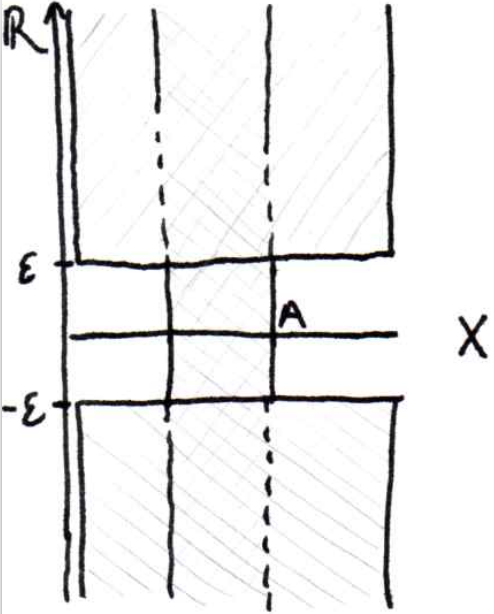
\includegraphics[scale=0.3]{produkt3e.png}
		\caption{Prostor W}
		\label{fig:prW}
	\end{figure}
	
	Najprej označimo $W = X \times (-\infty, -\epsilon] \cup X \times [\epsilon, \infty) \cup A \times \R$, $U = X \times (-\infty, -\epsilon] \cup A\times \R$ in $V = X \times [\epsilon, \infty) \cup A \times \R$ (skica \ref{fig:prW}). Ta zapis bomo pretvorili v notacijo, ki ustreza aksiomu o izrezu, ki nam bo tako kot v definiciji (predgovoru) izrezne triade zagotovil želeni izomorfizem. Najprej definiramo $Z = U \setminus V = (X \setminus A) \times (-\infty, -\epsilon]$. Oglejmo si zaporedje inkluzij $Z \subset U \subset W$. Velja $W \setminus U = (X \setminus A) \times [\epsilon, \infty)$. Zanima nas, ali obstaja zvezna preslikava $\tau\colon W \to [0, 1]$, da je $\tau|_Z \equiv 0$ in $\tau|_{W\setminus U} \equiv 1$. To preslikavo zlahka skonstruiramo (skica \ref{fig:tau3e})
	\[
	\tau(x, t) = \begin{cases}
	0 ; \; t \leq -\epsilon \\
	\frac{t + \epsilon}{2\epsilon} ; \; t \in [-\epsilon, \epsilon]\\
	1 ; \; t \geq \epsilon
	\end{cases}
	\]
	
	\begin{figure}[h]
		\centering
		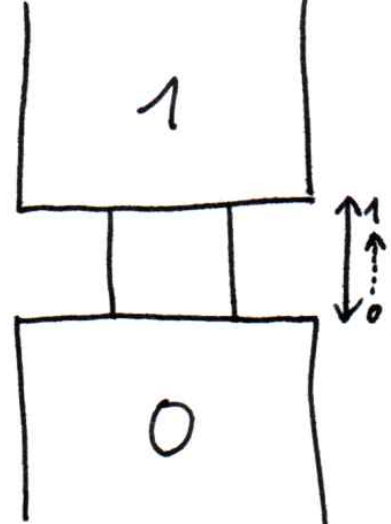
\includegraphics[scale=0.3]{preslikava3e.png}
		\caption{Preslikava $\tau$}
		\label{fig:tau3e}
	\end{figure}
	
	\item Privzemimo, da je $A \subset X$ odprta množica in da obstaja zvezna preslikava $\varphi \colon \closure{A} \to [0, 1]$, da je $\varphi(A) \subset (0, 1]$ in $\varphi(\partial A) = 0$. Radi bi dokazali, da je $(X \times (-\infty, 0) \cup X \times (0, \infty) \cup A \times \R;  X \times (-\infty, 0) \cup A\times \R, X \times (0, \infty) \cup A \times \R)$ izrezna triada za vsako homološko teorijo $h_*$.
	
	Vzemimo notacijo iz prejšnje naloge (le $\epsilon$ pošljemo proti $0$). Opazimo, da nam preslikava $\varphi$ na nek način meri oddaljenost od $\partial A$ znotraj množice $A$, saj ima $\varphi$ vrednost $0$ natanko na $\partial A$. Skonstruiramo naslednjo preslikavo 
	\[
	\tau(x, t) = \begin{cases}
	0 ; \; (x, t) \in (X \setminus A) \times (-\infty, 0) \\
	\varphi(x) ; \; (x, t) \in \closure{A} \times (-\infty, 0) \setminus K\\
	H_t(x) ; \; (x, t) \in \closure{K} \cap X\\
	1 - \varphi(x) ; \; (x, t) \in \closure{A} \times (0, \infty) \setminus K\\
	1 ; \; (x, t) \in (X \setminus A) \times (0, \infty)
	\end{cases}
	\]
	kjer je $K$ odprta krogla v produktu, ki jo skonstruiramo okoli nivoja $A\times\lbrace 0 \rbrace$, za razdaljo pa uporabimo funkcijo $\varphi$, $H$ pa je homotopija med funkcijama $\varphi$ in $1 - \varphi$, ki preči čez $K$.
	Konkretno, definiramo "kroglo"
	\[
	K = \lbrace (x, t) \in A\times \R ; \; |t| < \varphi(x) \rbrace
	\]
	in preslikavo $H \colon K \to [0, 1]$ s predpisom
	\[
	H(x, t) = \frac{(1 - 2\varphi(x))t + \varphi(x)}{2\varphi(x)}.
	\]
	Tukaj za vsak $x \in A$ velja $t \in [-\varphi(x), \varphi(x)]$.
	To je dobro definirano, ker je $A$ odprta množica in zato množica $K$ ne vsebuje njenih robnih točk na nivoju $t = 0$, kjer bi imeli težave z zveznostjo (skica \ref{fig:tau3f}).
	
	\begin{figure}[h]
		\centering
		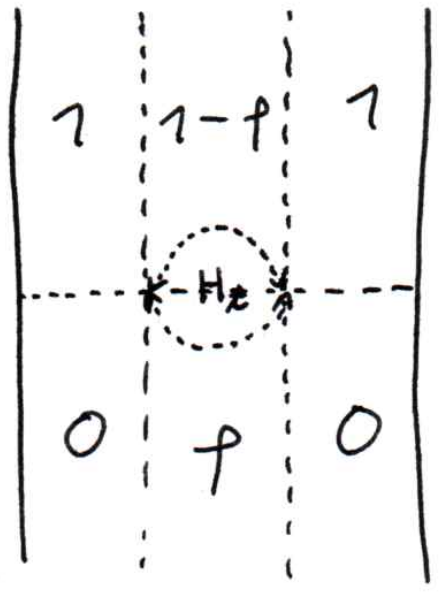
\includegraphics[scale=0.3]{preslikava3f.png}
		\caption{Preslikava $\tau$}
		\label{fig:tau3f}
	\end{figure}
	
	Naslednje tri rešitve bodo v veliki meri odvisne od konstrukcije homologije s cikli in mejami na račun aksiomatičnosti.
	\item Naj bosta $J_+$ in $J_-$ intervala, uporabljena pri prejšnjih dveh točkah. Dokažimo, da je
	\[
	\Delta_n\colon h_n(X \times \R, X \times (J_+ \cup J_-) \cup A \times \R) \to h_{n-1}(X \times \R, A \times \R)
	\]
	(preslikava iz točke (c)) izomorfizem.
	
	Po eksaktnosti dolgega zaporedja iz točke (c) je to ekvivalentno temu, da sta
	\begin{align*}
	&\varphi_n \colon h_n(X\times\R, A\times\R) \to h_n(X\times\R, X\times J_- \cup A\times\R)\oplus h_n(X\times\R, X\times J_+ \cup A\times\R)\\
	&\psi_n\colon h_n(X\times\R, X\times J_- \cup A\times\R)\oplus h_n(X\times\R, X\times J_+ \cup A\times\R) \to h_n(X\times\R, X\times (J_- \cup J_+) \cup A \times \R)
	\end{align*}
	ničelni preslikavi.
	%Preslikava $\varphi_n$ je ničelna, saj je $X \times J_- \cup A \times \R \htpeq A \times \R \htpeq X \times J_+ \cup A \times \R$ na povezanih komponentah, kjer $A$ obstaja, sicer pa je komponenta homotopna točki, saj je $\R$ kontraktibilen prostor. Imamo torej situacijo $G \to G \oplus G$ z dvema inkluzijama (ena z minusom), torej
	
	Preslikava $\varphi_n$ je ničelna, saj je inducirana z inkluzijama in je vsak cikel iz domene homotopen ciklu vsakega od členov vsote, saj je $X\times \R \htpeq X \times J_- \htpeq X \times J_+$, taki cikli pa so v obeh grupah vsote trivialni. Preslikava $\psi_n$ je ničelna iz istega razloga.
	
	\item Dokažimo še, da projekcija $(X \times \R, A \times \R) \to (X, A)$ inducira izomorfizem in da posledično obstaja izomorfizem $\sigma\colon h_{n-1}(X, A) \to h_n(X\times\R, X\times (J_+ \cup J_-) \cup A \times \R)$, ki je funktorialen v $(X, A)$.
	
	Projekcija seveda inducira zgornji izomorfizem, saj je $\R$ kontraktibilen prostor. Konkretno je $(X \times \R, A \times \R) \htpeq (X, A)$ s projekcijsko preslikavo, torej je po aksiomu o homotopiju inducirana preslikava izomorfizem.
	Od tod potem iz prejšnje točke sledi $h_{n}(X\times\R, W) \iso h_{n-1}(X\times\R, A\times\R) \iso h_{n-1}(X, A)$, kar preberemo iz desne proti levi za željeni izomorfizem, ki je funktorialen v $(X, A)$, saj je vmesni vezni morfizem definiran z veznim morfizmom para, ki pa je (kot smo videli pri točkah (b) in (c)) naravna transformacija, projekcijska preslikava pa je prav tako funktorialna.
	
	\item Za konec naloge identificirajmo še morfizem $h_n(X\times\R, X\times (J_+ \cup J_-) \cup A \times \R) \to h_n(X\times\R, X\times (J_+ \cup J_-) \cup A\times\R)$, ki ga inducira preslikava $(x, t) \mapsto (x, -t)$ na $X\times\R$.
	
	Ta morfizem je identičen. Če sta $J_+$ in $J_-$ kot v točki (f), je to očitno, saj so edini netrivialni cikli na osi $X \times \lbrace 0 \rbrace$, kjer je preslikava $(x, t) \mapsto (x, -t)$ identična. Če sta $J_+$ in $J_-$ kot v točki (e), je zaradi simetrije v prostoru vsak netrivialen del cikla homotopen simetričnemu ciklu (glede na os $X\times\lbrace 0 \rbrace$), ki pa se s preslikavo slika sam vase, torej je inducirani morfizem zopet identičen.
\end{enumerate}

\underline{\textbf{Nal. 4:}}
Naj bosta $p$ in $q$ tuji si naravni števili. Naj bo $f\colon\S^2_+ \to \S^2_-$ podana s predpisom $f(x, y, z) = (R(x, y), z)$, kjer je $R$ rotacija za kot $2\pi\frac{q}{p}$. Opazimo, da brez škode splošnosti privzamemo $q \leq p$. Naj bo $\sim$ najmanjša ekvivalenčna relacija na $\B^3$, da je $(x, y, z) \sim f(x, y, z)$ za vse $(x, y, z) \in \S^2_+$. Naj bo $L^3(p, q) = \B^3 / \sim$.

\begin{enumerate}[label=(\alph*)]
	\item Najprej pokažimo, da je $L^3(p, q)$ mnogoterost. Spomnimo se trditve iz Uvoda v geometrijsko topologijo, ki pravi, da za zvezno in zaprto surjekcijo $q \colon X \to Y$ velja: če je $X \in T_2$ in so vlakna preslikave $q$ kompaktna, je tudi $Y \in T_2$. Naša kvocientna projekcija $\pi \colon \B^3 \to L^3(p, q)$ je očitno zvezna in zaprta surjekcija, njena vlakna pa so končne unije točk, torej kompaktne množice. Prostor $L^3(p, q)$ je tudi $2$-števen, saj se števna baza prostora $\B^3$ direktno prenese na $L^3(p, q)$ preko preslikave $\pi$. Če je $\lbrace (U, \varphi) \rbrace$ atlas na mnogoterosti $\B^3$, je $\lbrace (\pi(U), \bar{\varphi}) \rbrace$ atlas na $L^3(p, q)$, kjer je $\bar{\varphi}$ inducirana preslikava preslikavi $\varphi$ preko kvocientne preslikave $\pi$.
	\item Preverimo še, da $L^3(p, q)$ dopušča CW-strukturo. Najlažje jo je kar sestaviti; dobimo eno $3$-celico $D$, eno $2$-celico $\sigma$, eno $1$-celico $a$ in eno $0$-celico $P$. Lepilne preslikave si bomo ogledali kasneje, pri računanju homoloških grup.
	
	\begin{figure}[h]
		\centering
		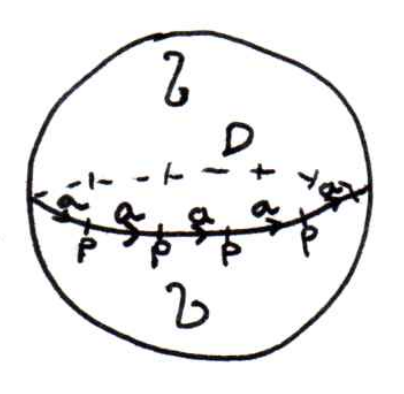
\includegraphics[scale=0.4]{cw4b.png}
		\caption{CW-struktura na $L^3(p, q)$}
		\label{fig:cw4b}
	\end{figure}
	
	\item Izračunajmo fundamentalno grupo $\pi_1(L^3(p, q))$. Spomnimo se, da je za fundamentalno grupo pomemben le skelet do dimenzije $2$. Razvidno je edina netrivialna zanka cikel $a$, hkrati pa vemo, da je ekvatorska zanka, ki je zaradi tujosti števil $p$ in $q$ sestavljena iz $p$-mnogo ciklov $a$, trivialna. Tako dobimo
	\[
	\pi_1(L^3(p, q)) = < a \; | \; a^p > \iso \Z_p.
	\]
	\item Izračunajmo še homološke grupe $H_*(L^3(p, q))$. Iz zgornje CW-strukture dobimo verižni kompleks
	\[
	0 \xrightarrow{} \Z(D) \xrightarrow{d_3} \Z(\sigma) \xrightarrow{d_2} \Z(a) \xrightarrow{d_1} \Z(P) \xrightarrow{} 0
	\]
	Oglejmo si označene preslikave. Očitno je $d_1(a) = 0$, zato je $d_1 \equiv 0$. Vemo $d_2(\sigma) = da$, kjer je $d = \deg\left(\S^1 \to X^{(1)} \to X^{(1)} / (X^{(1)}\setminus \mathring{a}) \homeo \S^1\right)$. Ta preslikava je $z \mapsto z^p$, zato je $d = p$ in $d_2(\sigma) = pa$. Opazimo, da je $d_2$ injektivna preslikava. Dalje je $d_3(D) = d\sigma$, kjer je $d = \deg\left(\S^2 \to X^{(2)} \to X^{(2)} / (X^{(2)}\setminus \mathring{\sigma}) \homeo \S^2\right)$. Zaradi vmesnega zrcaljenja je $d = 1 - 1 = 0$ in zato $d_3 \equiv 0$.
	
	Od tod dobimo 
	\begin{align*}
	H_0(L^3(p, q)) &= \Z(P) / \im d_1 = \Z(P) \iso \Z \\
	H_1(L^3(p, q)) &= \ker d_1 / \im d_2 = \Z(a) / p\Z(a) = \Z_p(a) \iso \Z \\
	H_2(L^3(p, q)) &= \ker d_2 / \im d_3 \iso 0 \\
	H_3(L^3(p, q)) &= \ker d_3 = \Z(D) \iso \Z
	\end{align*}
	\item Za katere $p, q$ je $L^3(p, q)$ orientabilna mnogoterost? Za $p = q = 1$, sicer vsebuje očiten M\"obiusov trak.
\end{enumerate}

\underline{\textbf{Nal. 5:}}
Naj bo $X$ pravilni dvanajsterec. Na ploskvah (dvanajst pravilnih petkotnikov) definiramo najmanjšo ekvivalenčno relacijo $\sim$, da je $x \sim f_D(x)$, kjer je $f_D \colon D \to D'$ homeomorfizem, ki je kompozitum rotacije za $36^\circ$. Označimo $S = X/_\sim$.

\begin{enumerate}[label=(\alph*)]
	\item Najprej pokažimo, da je $S$ mnogoterost. Enako kot pri nalogi $4$a je kvocientna projekcija $\pi \colon X \to X/_\sim$ očitno zaprta (in odprta) surjekcija, iz česar sledi, da je $S$ Hausdorffov in $2$-števen prostor (enako kot prej). Notranje okolice se vse ohranijo. Vsaka robna okolica se slika v končno mnogo kopij same sebe, torej je za $\lbrace (U, \varphi) \rbrace$ atlas na $X$ družina $\lbrace (\pi(U), \overline{\varphi})$ atlas na $S$.
	\item Pokažimo, da $S$ dopušča CW-strukturo. Zopet jo bo najlažje kar sestaviti \footnote{Slika (seveda brez barvanj) je dostopna na \url{https://www.timvandevall.com/printable-paper-dice-template/}}.
	\begin{figure}[h]
		\centering
		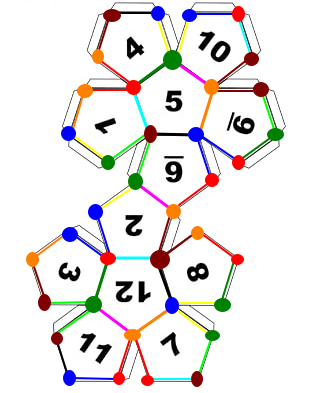
\includegraphics[scale=0.6]{cw5b.png}
		\caption{Relacije na $S$}
		\label{fig:cw5}
	\end{figure}
	
	Dobimo eno $3$-celico $D$, ki predstavlja notranjost dvanajsterca in je na sliki ne vidimo, šest $2$-celic $\sigma_1, \dots, \sigma_6$, ki jih zaporedoma predstavljajo pari ploskev $(1, 7), (2, 10), (3, 9), (4, 8), (5, 12), (6, 11)$. Glede na robove ploskev dobimo deset $1$-celic: $a$ (rdeča), $b$ (oranžna), $c$ (rumena), $d$ (svetlo zelena), $e$ (svetlo modra), $f$ (temno modra), $g$ (vijolična), $h$ (rjava), $i$ (temno zelena) in $j$ (črna). Nazadnje dobimo še pet $0$-celic: $P_1, \dots, P_5$, zaporedoma označenih z rdečo, oranžno, temno modro, temno zeleno in rjavo barvo. Orientacija bo določena kasneje, pri izračunu homologije, načeloma pa je rob ploskve $1$ orientiran pozitivno, ploskve $2$ negativno, ploskev $4$ pa ima v pozitivni smeri rob $i - c - j - h - a$ (kar nam že določi orientacijo robov vseh ploskev).
	
	\item Ker je za fundamentalno grupo pomemben le skelet do dimenzije $2$, dobimo z upoštevanjem relacij naslednjo grupo
	\[
	\pi_1(S) = < a, b, c, d, e, f, g, h, i, j \; | \; abcde, cghef, bf^{-1}idh^{-1}, ahjci^{-1}, bj^{-1}eig, ag^{-1}djf^{-1}>,
	\]
	dalje pa je ne bomo poenostavljali.
	
	\item Izračunajmo homološke grupe $H_*(S)$. Oglejmo si verižni kompleks
	\[
	0 \xrightarrow{} \Z(D) \xrightarrow{d_3} \Z(\sigma_1, \dots, \sigma_6) \xrightarrow{d_2} \Z(a, \dots, j) \xrightarrow{d_1} \Z(P_1, \dots, P_5) \xrightarrow{} 0
	\]
	Upoštevajoč relacije dobimo matrike preslikav
	\[
	d_1 = \begin{bmatrix}
	-1 & 0 & 0 & 0 & 1 & -1 & 0 & 0 & -1 & 0 \\
	1 & -1 & 0 & 0 & 0 & 0 & 1 & -1 & 0 & 0\\
	0 & 1 & -1 & 0 & 0 & 1 & 0 & 0 & 0 & -1\\
	0 & 0 & 1 & -1 & 0 & 0 & -1 & 0 & 1 & 0\\
	0 & 0 & 0 & 1 & -1 & 0 & 0 & 1 & 0 & 1
	\end{bmatrix},
	\]
	\[
	d_2 = \begin{bmatrix}
	1 & 0 & 0 & -1 & 0 & -1 \\
	1 & 0 & -1 & 0 & -1 & 0 \\
	1 & -1 & 0 & -1 & 0 & 0 \\
	1 & 0 & -1 & 0 & 0 & -1 \\
	1 & -1 & 0 & 0 & -1 & 0 \\
	0 & -1 & 1 & 0 & 0 & 1 \\
	0 & -1 & 0 & 0 & -1 & 1 \\
	0 & -1 & 1 & -1 & 0 & 0 \\
	0 & 0 & -1 & 1 & -1 & 0 \\
	0 & 0 & 0 & -1 & 1 & -1
	\end{bmatrix}
	\]
	in zaradi translacij $d_3 \equiv 0$ (rotacija ne prispeva nič, translacija pa je tukaj podobna zrcaljenju).
	S pomočjo računalnika izračunamo, da je jedro matrike $d_1$ enako $\ker d_1 = \Z(a - d - e, b + c + d + e + f, -b -c + g, c + d + h, -c - d - e + i, - b - c - d + j)$, njena slika pa je $\im d_1 = \Z(-P_1 + P_2, -P_2 + P_3, -P_3 + P_4, -P_4 + P_5)$. Podobno dobimo $\ker d_2 = 0$ in $\im d_2 = \Z(a + b + c+ d + e, -c - e - f - g - h, -b - d + f + h - i, -a - c - h + i - j, -b - e - g - i + j, - a - d + f + g - j)$, z drugimi besedami, matrika $d_2$ ima poln rank.
	Od tod s spremembo baze hitro sledi
	\[
	H_0(S) = \Z(P_1, \dots, P_5) / \Z(-P_1 + P_2, -P_2 + P_3, -P_3 + P_4, -P_4 + P_5) \iso \Z(P_1)
	\]
	Dobimo tudi
	\[
	H_2(S) = \ker d_2 / \im d_3 = 0
	\]
	in seveda
	\[
	H_3(S) = \ker d_3 = \Z(D)
	\]
	Na koncu s spremembo baze dobimo tudi
	\[
	H_1(S) = \ker d_1 / \im d_2 = 0
	\]
\end{enumerate}


\underline{\textbf{Nal. 7:}}
Naj bo $0 \leq k \leq n$ in naj bo $i \colon \I^k \to \S^n$ vložitev. Pokažimo, da za reducirano homologijo velja $\widetilde{H}_*(\S^n \setminus i(\I^k)) = 0$.

Najprej se spomnimo pojma reducirane homologije. Reducirana homologija verižnega kompleksa $C_\bullet$ je homologija t.i. augmentiranega kompleksa
\[
\cdots \xrightarrow{} C_n \xrightarrow{} \cdots \xrightarrow{} C_1 \xrightarrow{} C_0 \xrightarrow{\epsilon} \Z \xrightarrow{} 0,
\]
kjer je $\epsilon (\Sigma_i n_i \sigma_i) = \Sigma_i n_i$. Ključna lastnost reducirane homologije je, da so vse reducirane homološke grupe prostora z eno točko trivialne (pri običajni homologiji dobimo v dimenziji $0$ grupo $\Z$). Opazimo, da za $n > 0$ velja $H_n = \widetilde{H}_n$, za $n = 0$ pa imamo $H_0 = \ker\epsilon / \im d_1$. Spomnimo se tudi, da imajo homotopni prostori izomorfne homološke grupe, zato je na primer vsaka reducirana homološka grupa $n$-razsežnega diska (odprtega ali zaprtega) prav tako trivialna.

Nalogo bomo rešili z indukcijo na $k$ za fiksen $n$.
\begin{itemize}
	\item \underline{$k=0$:} Ker je $\I^0 \homeo \lbrace * \rbrace$ (prostor z eno točko), je $\widetilde{H}_*(\S^n\setminus i(\I^0)) \iso \widetilde{H}_*(\mathring{\B}^n) \iso \widetilde{H}_*(\lbrace * \rbrace)$, torej je $\widetilde{H}_n(\S^n \setminus i(\I^0)) = 0$ za vsak $n \geq 0$.
	\item \underline{$k-1 \to k$:} Zapišimo $\I^k = K_1 \cup K_2$, kjer sta $K_1, K_2$ ravno zaprta kvadra, ki delita $\I^k$ na polovico, in velja $K_1 \cap K_2 = \I^{k-1}\times \lbrace \frac{1}{2} \rbrace$. Zaradi injektivnosti preslikave $i$ opazimo, da je $X = \S^n\setminus i(\I^k) = (\S^n \setminus i(K_1)) \cap (\S^n \setminus i(K_2))$ in $(\S^n \setminus i(K_1)) \cup (\S^n \setminus i(K_2)) = \S^n \setminus i(K_1 \cap K_2) \homeo \S^n \setminus i(\I^{k-1})$, kar nam da dobro podlago za uporabo Mayer-Vietorisovega dolgega zaporedja. Konkretno, za vsak $l \geq 0$ imamo
	\[
	\cdots \xrightarrow{} \widetilde{H}_{l+1}(\S^n \setminus i(\I^{k-1})) \xrightarrow{} \widetilde{H}_l(X) \xrightarrow{} \widetilde{H}_l(\S^n \setminus i(K_1)) \oplus \widetilde{H}_l(\S^n \setminus i(K_2)) \xrightarrow{} \widetilde{H}_l(\S^n \setminus i(\I^{k-1})) \xrightarrow{} \cdots
	\]
	Ker je $K_1 \homeo K_2 \homeo \I^k$, je $i(K_1) \homeo i(K_2) \homeo i(\I^k)$ ($i$ je zvezna, zaprta in 1-1). Označimo $G = \widetilde{H}_l(X)$ in upoštevamo indukcijsko predpostavko, da dobimo
	\[
	0 \xrightarrow{} G \xrightarrow{} G \oplus G \xrightarrow{} 0.
	\]
	Imamo torej $G \iso G \oplus G$, kjer je ta izomorfizem, induciran s parom inkluzij, enak $\alpha \mapsto (\alpha, -\alpha)$. To je v nasprotju z bijektivnostjo, ker ta preslikava jasno ni surjektivna, razen v primeru, ko je $G$ trivialna grupa. Dokaz z indukcijo je s tem končan.
\end{itemize}

\underline{\textbf{Nal. 8:}}
Oglejmo si vozel na sliki \ref{fig:vozel} in izračunajmo njegovo fundamentalno grupo.
\begin{figure}[h]
	\centering
	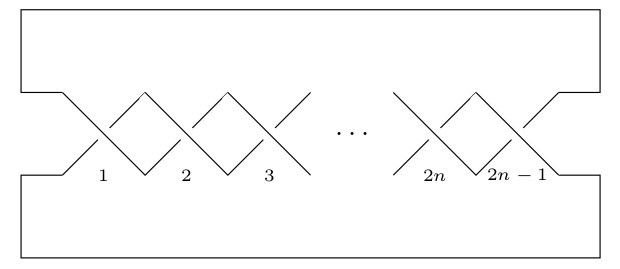
\includegraphics[scale=0.4]{knot8.png}
	\caption{Vozel $K_n$ v $\R^3$ (namesto $2n-1$ bi moralo pisati $2n+1$).}
	\label{fig:vozel}
\end{figure}

Najprej levo zgoraj v vsakem križišču dobimo generatorje $a_1,\dots, a_{2n+1}$, vsak od njih sega nad vozlom in je kot puščica usmerjen diagonalno od levo spodaj do desno zgoraj. Nato izračunamo relatorje s sprehodom pod vsakim križiščem začenši na zahodnji točki, premikamo pa se v smeri urinega kazalca. Zaporedni relator na $k$-tem križišču je tako oblike $a_{k-1}a_{k}^{-1}a_{k+1}^{-1}a_{k}$ (indekse priredimo za robna križišča po modulu). Dobimo naslednjo fundamentalno grupo
\[
\pi_1(K_n) = < a_1, a_2, \dots, a_{2n},\; a_{2n+1} \; | \; a_{2n+1}a_1^{-1}a_2^{-1}a_1, a_1a_2^{-1}a_3^{-1}a_2, \dots, \; a_{2n-1}a_{2n}^{-1}a_{2n+1}^{-1}a_{2n},\; a_{2n}a_{2n+1}^{-1}a_{1}^{-1}a_{2n+1}  >
\]
Poskusimo poenostaviti relatorje in se znebiti nekaterih generatorjev. Iz prvega relatorja dobimo
\[
a_{2n+1} = a_1^{-1}a_2a_1.
\]
Sedaj se lotimo relatorjev iz zadnje strani. ($2n+1$)-i relator nam da enakost
\[
a_{2n} = a_{2n+1}^{-1}a_1a_{2n+1} = a_1^{-1}a_2^{-1}a_1a_1a_1^{-1}a_2a_1 = (a_2a_1)^{-1}a_1(a_2a_1),
\]
$2n$-ti nam posledično da enakost
\[
a_{2n-1} = \cdots = (a_1a_2a_1)^{-1}a_2(a_1a_2a_1).
\]
Tako nadaljujemo in induktivno dobimo
\begin{align*}
	a_{2k} &= ((a_2a_1)^{n-k+1})^{-1}a_1(a_2a_1)^{n-k+1} \\
	a_{2k-1} &= (a_1(a_2a_1)^{n-k+1})^{-1}a_2(a_1(a_2a_1)^{n-k+1})
\end{align*}
za indekse večje od $2$.
Iz tretjega in drugega relatorja potem zaporedoma sledi tudi
\begin{align*}
a_{2} &= ((a_2a_1)^{n-1})^{-1}a_1(a_2a_1)^{n-1} \\
a_{1} &= (a_1(a_2a_1)^{n})^{-1}a_2(a_1(a_2a_1)^{n})
\end{align*}
Ko obe enačbi preuredimo tako, da je na levi strani $1$, izpostavimo komutator na sredini in ga nato nesemo na levo stran enačbe, vidimo, da sta obe zgornji enačbi ekvivalentni enačbi
\[
[a_1, a_2] = (a_2(a_1a_2)^{n-1})\cdot(a_1(a_2a_1)^{n-1})^{-1},
\]
kar pomeni, da je fundamentalna grupa vozla $K_n$ enaka
\[
\pi_1(K_n) = < a_1, a_2 \; | \; (a_2(a_1a_2)^{n-1})^{-1}[a_1, a_2](a_1(a_2a_1)^{n-1}) >,
\]
kjer definiramo $[g, h] = g^{-1}h^{-1}gh$.

Radi bi tudi videli, da za $n \neq m$ vozla $K_n$ in $K_m$ nista ekvivalentna, za kar pa zadostuje pokazati, da grupi $\pi_1(K_n)$ in $\pi_1(K_m)$ nista izomorfni za $n \neq m$.

Takoj opazimo, da je v $K_0$ (eno križišče) en sam generator $a_1$, torej $\pi_1(K_0) \iso \Z$, kar je komutativna grupa (iz skice je prav tako očitno, da z enim polobratom spodnjega dela vozel $K_0$ pretvorimo v $\S^1$). Ostalim grupam komutator hitro raste, torej niso komutativne in zato niso izomorfne $\pi_1(K_0)$. Še več, ker se z izomorfizmom center grupe slika v center (komplement centra pa v komplement), grupi za $n \neq m$ ne moreta biti izomorfni.

\end{document}

%% TEMPLATES
% lists
%\begin{enumerate}[label=(\alph*)]
% diagram
%\adjustbox{scale=1, center}{
%	\begin{tikzcd}
%		\R_n \arrow[d, "\varphi_n"] \arrow[r, "\Phi"] & \R_m \arrow[d, "\varphi_m"] \\
%		\R \arrow[r, "\widetilde{\Phi}"] & \R
%	\end{tikzcd}
%}
% figure
%\begin{figure}[h]
%	\centering
%	\includegraphics[scale=0.4]{fig}
%	\caption{caption}
%	\label{fig:label}
%\end{figure}
